\documentclass[oneside,a4paper,10pts,article]{memoir}
\usepackage[utf8]{inputenc}

\usepackage[danish]{isodate}

\usepackage{palatino}
\usepackage{graphicx}
\usepackage{todonotes}
\presetkeys{todonotes}{inline}{}

\usepackage{url}
\usepackage[hidelinks,hyperindex]{hyperref}

\captionnamefont{\bfseries}

\usepackage{tikz}
\usetikzlibrary{positioning,arrows,calc}

\newcommand{\vs}{%
    \tikz[remember picture,overlay]{\node at
        ($(current page.south east)+(-2,2)$)
        [anchor=south east] {Vend siden $\rightarrow$};}
}

\usepackage{listings}
\lstdefinelanguage{JavaScript}{
  keywords={break, case, catch, continue, debugger, default, delete,
    do, else, false, finally, for, function, if, in, instanceof, new,
    null, return, switch, this, throw, true, try, typeof, var, void,
    while, with},
  morecomment=[l]{//},
  morecomment=[s]{/*}{*/},
  morestring=[b]',
  morestring=[b]",
  ndkeywords={class, export, boolean, throw, implements, import, this},
  keywordstyle=\color{blue},
  ndkeywordstyle=\color{darkgray},
  identifierstyle=\color{black},
  commentstyle=\color{purple}\ttfamily,
  stringstyle=\color{red}\ttfamily,
  sensitive=true,
  extendedchars=true,
literate=%
{æ}{{\ae}}1
{å}{{\aa}}1
{ø}{{\o}}1
{Æ}{{\AE}}1
{Å}{{\AA}}1
{Ø}{{\O}}1
}

\lstset{
  basicstyle=\ttfamily\footnotesize,
  keywordstyle=\bfseries,
  captionpos=b,
  language=JavaScript
}

% Remove section numbers
\setsecnumdepth{part}

% Remove page numbers
\renewcommand\thepage{}

\title{Animation i Processing
  \\ {\normalfont\small\scshape Coding Pirates DIKU }} \date{\today}

\begin{document}
\maketitle
\vs
\vspace{-10mm}
\chapter{Byg en by!}
Først en bil:
\begin{lstlisting}
var bilBredde = 50;
var bil = function(xpos) {
    ... tegnekode til bil ...
    ... brug bilBredde ..
};

var x = bilBredde;
var hastighed = 3;
draw = function() {
    background(255, 255, 255);
    bil(x);
    x = x + hastighed;
    
    if (x + bilBredde > width) {
        hastighed = -3;
    }
};
\end{lstlisting}

\vspace{-3mm}
\chapter{Opgaver}
Så er det din opgave at lave resten!
\begin{itemize}
\item Gør så bilen vender om i venstre side af skærmen.
\item Tegn en vej.
\item Få en bil mere til at køre på vejen.
\item Få bilen til at ændre udseende når \texttt{hastighed} er negativ.
\item Hvad kan der ellers være i en by? Tegn og animér!
\end{itemize}

\hspace{20mm}
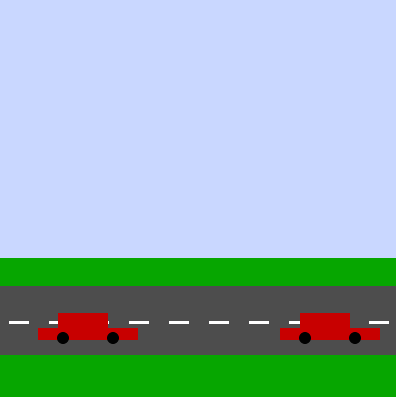
\includegraphics[width=0.35\textwidth]{pics/biler.png}

\newpage
\chapter{UFO-spil fortsat}


\chapter{Opgaver}
\begin{itemize}
\item 
\end{itemize}

\hspace{1cm}
% 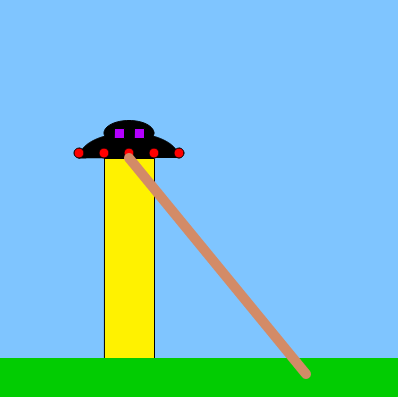
\includegraphics[width=0.4\textwidth]{pics/laserkanon.png}

\end{document}